%\subsection{Graphical User Interface}

\subsubsection*{Administration View}
\begin{figure}[!h]
	\centering
	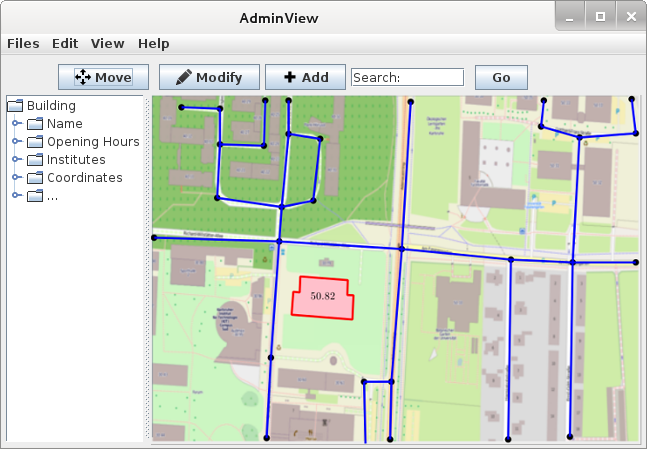
\includegraphics[scale=0.7]{gui-pictures/AdminView.png}
	\caption{Administration view with displayed \textit{routing graph}.}
\end{figure}
The administrator has the option to load and save the \textit{routing graphs} and
background images via the ``Files'' dialogue. In the toolbar below the main menu
will be a collection of tools for modifications of the \textit{routing graph} and
a \textit{search field} for specific locations.
On the right side will be a list of the selected nodes and edges with sub-entries of their
\textit{properties}. The main area shows the editable \textit{routing graph} of the \textit{map} and the \textit{background image}.

\begin{figure}[h!]
\begin{minipage}[hbt]{8cm}
	\centering
	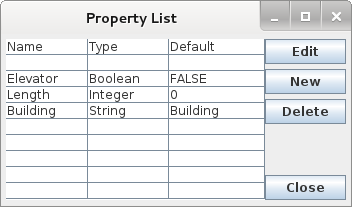
\includegraphics[scale=0.5]{gui-pictures/PropertyList.png}
	\caption{List of configured \textit{properties}.}
        \label{fig:propertyList}
\end{minipage}
\hfill
\begin{minipage}[hbt]{8cm}
	\centering
	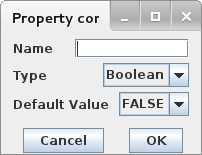
\includegraphics[scale=0.5]{gui-pictures/PropertyConfig.png}
	\caption{Configure a new \textit{property}.}
        \label{fig:propertyConfig}
\end{minipage}
\end{figure}

The \textit{property} list (Figure~\ref{fig:propertyList}) can be accessed through ``Edit --> Properties'' and will show a list of the names, datatypes and default values of
all available \textit{properties}, which can be added to vertices and edges. \\
To edit an entry in this list it has to be selected and then the ``Edit'' button pressed.
To add a new entry to the list the ``New'' button has to be pressed.
In each case a configuration dialogue (Figure~\ref{fig:propertyConfig}) will pop up, where the name, datatype and
default value can be entered.

\begin{figure}[h!]
\begin{minipage}[hbt]{8cm}
	\centering
	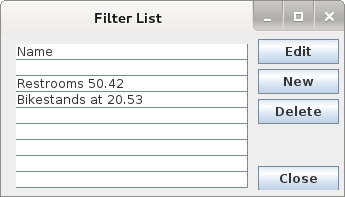
\includegraphics[scale=0.5]{gui-pictures/FilterList.png}
	\caption{List of configured filters.}
        \label{fig:filterList}
\end{minipage}
\hfill
\begin{minipage}[hbt]{8cm}
	\centering
	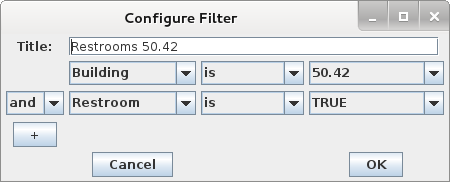
\includegraphics[scale=0.5]{gui-pictures/FilterConfig.png}
	\caption{Configure a filter.}
        \label{fig:filterConfig}
\end{minipage}
\end{figure}

Similar to the \textit{properties} filters will be shown and edited (Figures~\ref{fig:filterList} and~\ref{fig:filterConfig}).

\subsubsection*{Routing View}
\begin{figure}[!h]
	\centering
	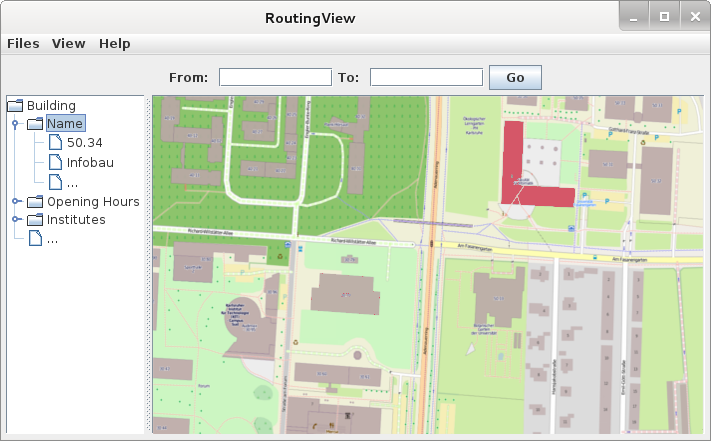
\includegraphics[scale=0.55]{gui-pictures/RoutingView.png} \\
	\caption{Routing view.}
\end{figure}
The routing view has two text fields labeled ``From'' and ``To'' for inserting
the start and endpoint of a route. The main area below shows the \textit{map} and the
calculated path of the route.
On the side of the \textit{map} will be a list of \textit{properties} of the current selection
(building, way, route, etc).

\newpage

\subsubsection*{View inside a building}
\begin{figure}[!h]
	\centering
	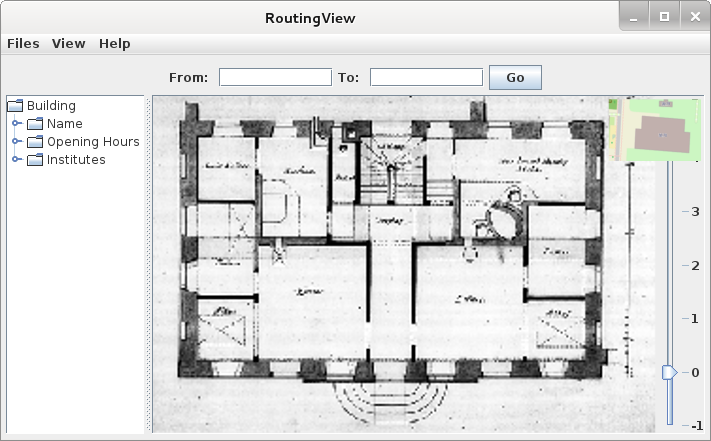
\includegraphics[scale=0.55]{gui-pictures/RoutingView_inside.png} \\
	\caption{Routing view inside a building.}
\end{figure}
The inside view of a building shows the \textit{floor plan map} of a building with an iconized
outside-map in a corner of the main map area. To change the displayed floor a
selection bar will be displayed at the right side.

To enter the building view a building has to be selected while a click on the mini-map or outside the outline of the building exits the building view.
